\scanpage{71}
% archive sheet number: 70

des \inserted{(iso)}\handwritten{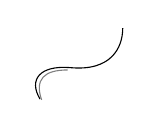
\begin{tikzpicture}[x=1cm,y=1cm,baseline=-.1cm]\draw[thin] (0,-.25).. controls (-.15,0) and (0,.18)..(.38,.15).. controls (.9,.1) and (1.05,.4)..(1.05,.65);\draw[gray,thin] (.02,-.26).. controls (-.07,0) and (.05,.12)..(.35,.12);\end{tikzpicture}}motifs \inserted{(semi-simples)}\handwritten{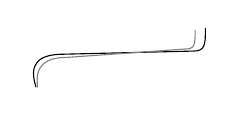
\begin{tikzpicture}[x=1cm,y=1cm,baseline=-.1cm]\draw[thin] (0,-.3).. controls (-.1,0) and (.03,.12)..(.35,.12)--(2,.16).. controls (2.15,.16) and (2.15,.25)..(2.15,.45);\draw[gray,thin] (.02,-.3).. controls (-.02,-.02) and (.12,.08)..(.4,.08)--(1.95,.19).. controls (2.02,.2) and (2.02,.3)..(2.02,.43);\end{tikzpicture}} sur $k$, et l'indice $\underline{Q}_p$ désigne l\unsure{\deleted{'}e|'e} \deleted{effet du} changement de base par $\underline{Q}\handwritten{\longrightarrow}\underline{Q}_p$ . Cet homomorphisme est compatible à l'augmentation ``de Tate'' et aux structures d'effectivité. Modulo du travail à faire de Berthelo\handwritten{t}, pour $k=\handwritten{\mathbb{F}}_q$ un corps fini à $q$ éléments, la connaissance de l'image \deleted{de $X$ d\unsure{q|a}n\unsure{s}} $H^*(X)$ dans $\mathrm{Fcriso}(k)$ permet de calculer \unsure{\deleted{s}l|\deleted{l}s}a fonction $\handwritten{\zeta_X}$ de $X$, par la formule qu'on devine et que je me dispose décrire. (D'ailleurs, modulo les conjectures de Weil, la connaissance de la fonction $\handwritten{\zeta_X}$ permet, grâce à cette formule, de réconstituer $H^{\handwritten{*}}_{\mathrm{cris}}(X)$ à isomorphisme près dans $\mathrm{Fcriso}(k)$, du moins virtuellement (i.e. l'image de chaque $H^i_{\mathrm{cris}}(X)$ dans l'anneau $K(\mathrm{Fcriso}(k)))$ si on ne désire pas admettre que \deleted{\unsure{l|t}\unsure{t|i|o}\unsure{o|u}\unsure{b|u|s}} les $H^i$ sont nécessairement des éléments semi-simples de $\mathrm{Fcriso}(k)$....)

\handwritten{5.} F-\uline{cristaux de \deleted{niveau} pente nulle}. On définira plus loin la \uline{pente} d'un F-cristal ``homogène''. Ici, nous allons \unsure{\deleted{o}i|\deleted{i}o}ntroduire directement les F-cristaux de pente nulle. Pour ceci, pour tout faisceau $p$-adique constructible \inserted{$V$}\handwritten{\begin{tikzpicture}[x=1cm,y=1cm,baseline=0cm]\draw[thin] (0,-.25).. controls (-.1,-.05) and (.3,.3)..(.4,.7);\end{tikzpicture}} sur $k$\handwritten{(}correspondant donc à une \deleted{repr\unsure{é|e}sentatio}n\inserted{opération} continue de $\handwritten{\pi}=\operatorname{Gal}(\handwritten{\bar{k}}/k)$ dans un module de type fini sur $\underline{Z}_p$) on lui associe de \deleted{\unsure{d|q}}\handwritten{f}açon évidente un F-cristal $M$, noté parfois (par abus de notations)
\[
M=\unsure{\mathbb{V}|\mathbb{M}|\mathbb{F}}\otimes_{\underline{Z}_p}W\ ,
\]
(même s'il n'y a pas de $W$ choisi, dans le cas $k$ imparfait \handwritten{!} ), \unsure{\deleted{o}O|\deleted{O}o|6}n aura :

\margin{\handwritten{\figure{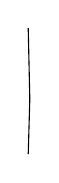
\begin{tikzpicture}\draw (0,0) -- (0.02,0.7) -- (0,1.6);\end{tikzpicture}}}}
\uline{Proposition}\handwritten{5\unsure{,|.}1.} Le foncteur $\mathbb{M}\handwritten{\mathrel{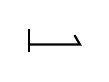
\begin{tikzpicture}[x=1cm,y=1cm,baseline=-.04cm]\draw[thick] (0,-.1)--(0,.2);\draw[thick] (0,0)--(.65,0)--(.58,.12);\end{tikzpicture}}}V\otimes_{\underline{Z}_p}W$ est une équivalence de la catégorie des faisceaux $p$-adiques constructibles\handwritten{\begin{tikzpicture}[x=1cm,y=1cm,baseline=0cm]\draw[thin] (0,-.3).. controls (.13,-.2) and (.14,.1)..(.26,.55);\end{tikzpicture}}sur $k$ vers la sous-catégorie pleine de la catégorie des F-cristaux \unsure{\deleted{d}s|\deleted{s}d}\unsure{\deleted{a}u|\deleted{u}a|\deleted{e}u|\deleted{u}e}r $k$, formée des F-cristaux $M$ tels que $F_M : M^{\handwritten{\unsure{\deleted{\sigma}\sigma|\sigma}}}\handwritten{\longrightarrow}M$ soit un \uline{isomorphisme} .

\uline{Corollaire}\handwritten{5.\unsure{2|1}.} Le foncteur précédent induit un foncteur pleinement fidèle (compatible avec les $\otimes$-structures)\inserted{\handwritten{$i$}}\handwritten{\begin{tikzpicture}[x=1cm,y=1cm,baseline=0cm]\draw[thin] (0,-.3).. controls (-.1,-.02) and (.2,.25)..(.5,.33).. controls (.7,.35) and (.85,.38)..(.95,.5);\end{tikzpicture}} de la catégorie des

\mspage{70}
